%%% Fiktivní kapitola s ukázkami tabulek, obrázků a kódu

\chapter{Řešítko}
Abychom mohli dokončit důkaz některých instancí hypotézy \ref{veta02:hypoteza}, potřebujeme získat požadované stavební bloky. Nabízí se naprogramovat řešítko, které bude umět alespoň některé typy hledaných grafů najít. Hlavním cílem této práce bylo takový program připravit a pomocí něj získat lepší představu o potenciálu uvedené konstrukce důkazu.

\section{Algoritmus}

Program na vstupu očekává zadání vnější stěny: každý vrchol je zastoupen jedním bitem, který určuje, zda má být ve výsledném grafu stupně 2 nebo 3. Navíc očekává seznam velikostí stěn, které má využít. Na výstupu informuje, zda se mu daný graf podařilo najít (říkejme \textbf{vyplnit}), a umožní jej exportovat.

Postup hledání původně imitoval lidské pokusy o řešení problému: nakreslit si vnější stěnu, zkusit spojit nějaké dva vrcholy řetízkem vhodné délky (aby nově uzavřená stěna byla z neutrální posloupnosti) a dokud je místo na papíře, spojovat. Pak si překreslit nejvnitřnější, zatím neuzavřenou stěnu (budeme mluvit o \textbf{hranici}), ta se stane \uv{vnější stěnou} na novém papíře a pokračovat. V situaci, kdy nelze dál nic spojit, nebo je jasné, že graf nemůže vyhovovat parametrům, vrátit se podle uvážení zpět. Viz obrázek TODO odkaz.

Kdybychom chtěli znát jen ano/ne odpověď, jestli graf existuje, nebylo by vůbec třeba si pamatovat celý rozpracovaný graf, stačilo-by pracovat s hranicemi, které navíc stačí reprezentovat jako binární číslo. Výsledkem by pak mohla být jen posloupnost hranic, kterými se prošlo před uzavřením grafu, nebo samotné \uv{ano/ne}. Překvapivě obtížné je pak z této posloupnosti nestrojově získat skutečný graf, proto program nabízí i možnost graf dodatečně rekonstruovat podle prošlých stavů.

V tento okamžik je jasné, že problém je vlastně prohledávání v binárních řetězcích (které reprezentují hranice). Je proto vhodné zmínit, podle jakého kritéria se program rozhoduje, kterým směrem hledat dále. Implementace vždy upřednostňuje ke zpracování již nalezený řetězec nejmenší délky, a pro něj najde všechny další sousedy.

Aby toto prohledávání fungovalo dobře, je třeba trochu zkomplikovat reprezentaci hranice. Hlavním požadavkem bude identita mezi reprezentací (jediným binárním řetězcem) a všemi hranicemi (tedy cykly, na kterých vyznačené vrcholy ještě vyžadují dalšího souseda), které jsou pro algoritmus izomorfní - tedy všechny rotace a převrácení hranice.

\begin{definice}[Hranice a její reprezentace]\label{def01:1}
Cyklus $C$ a množinu $I \subseteq C(V)$ zveme hranicí $H$. Množina $I$ jsou právě ty vrcholy, které ve výsledném vyplnění musí mít dalšího souseda. Pokud  $i = \emptyset$, mluvíme o hranici přímo jako o stěně.

Binární řetězec (číslo) reprezentující hranici $H$ získáme následně: každý vrchol H označíme buď znakem 1 (jako I v "in" podle orientace pomyslené hrany) nebo 0 (jako 0 v "out"). Zaznamenejme pak všechny řetězce, které získáme čtením od každého vrcholu pro i proti směru hodinových ručiček. Ten z nich, který z nich má největší hodnotu (pokud řetězec chápeme jako binární číslo), je reprezentací hranice. Pokud $i = \emptyset$, pak přidejme speciální znak a zapamatujme počet vrcholů.
\end{definice}

Pro lepší představu přikládáme posloupnost hranic s vizualizací na obrázku \ref{obr03:reseni}, která řeší (4,4,3)$\lbrace$4,7$\rbrace$-triark. 

\begin{figure}[h!]\centering
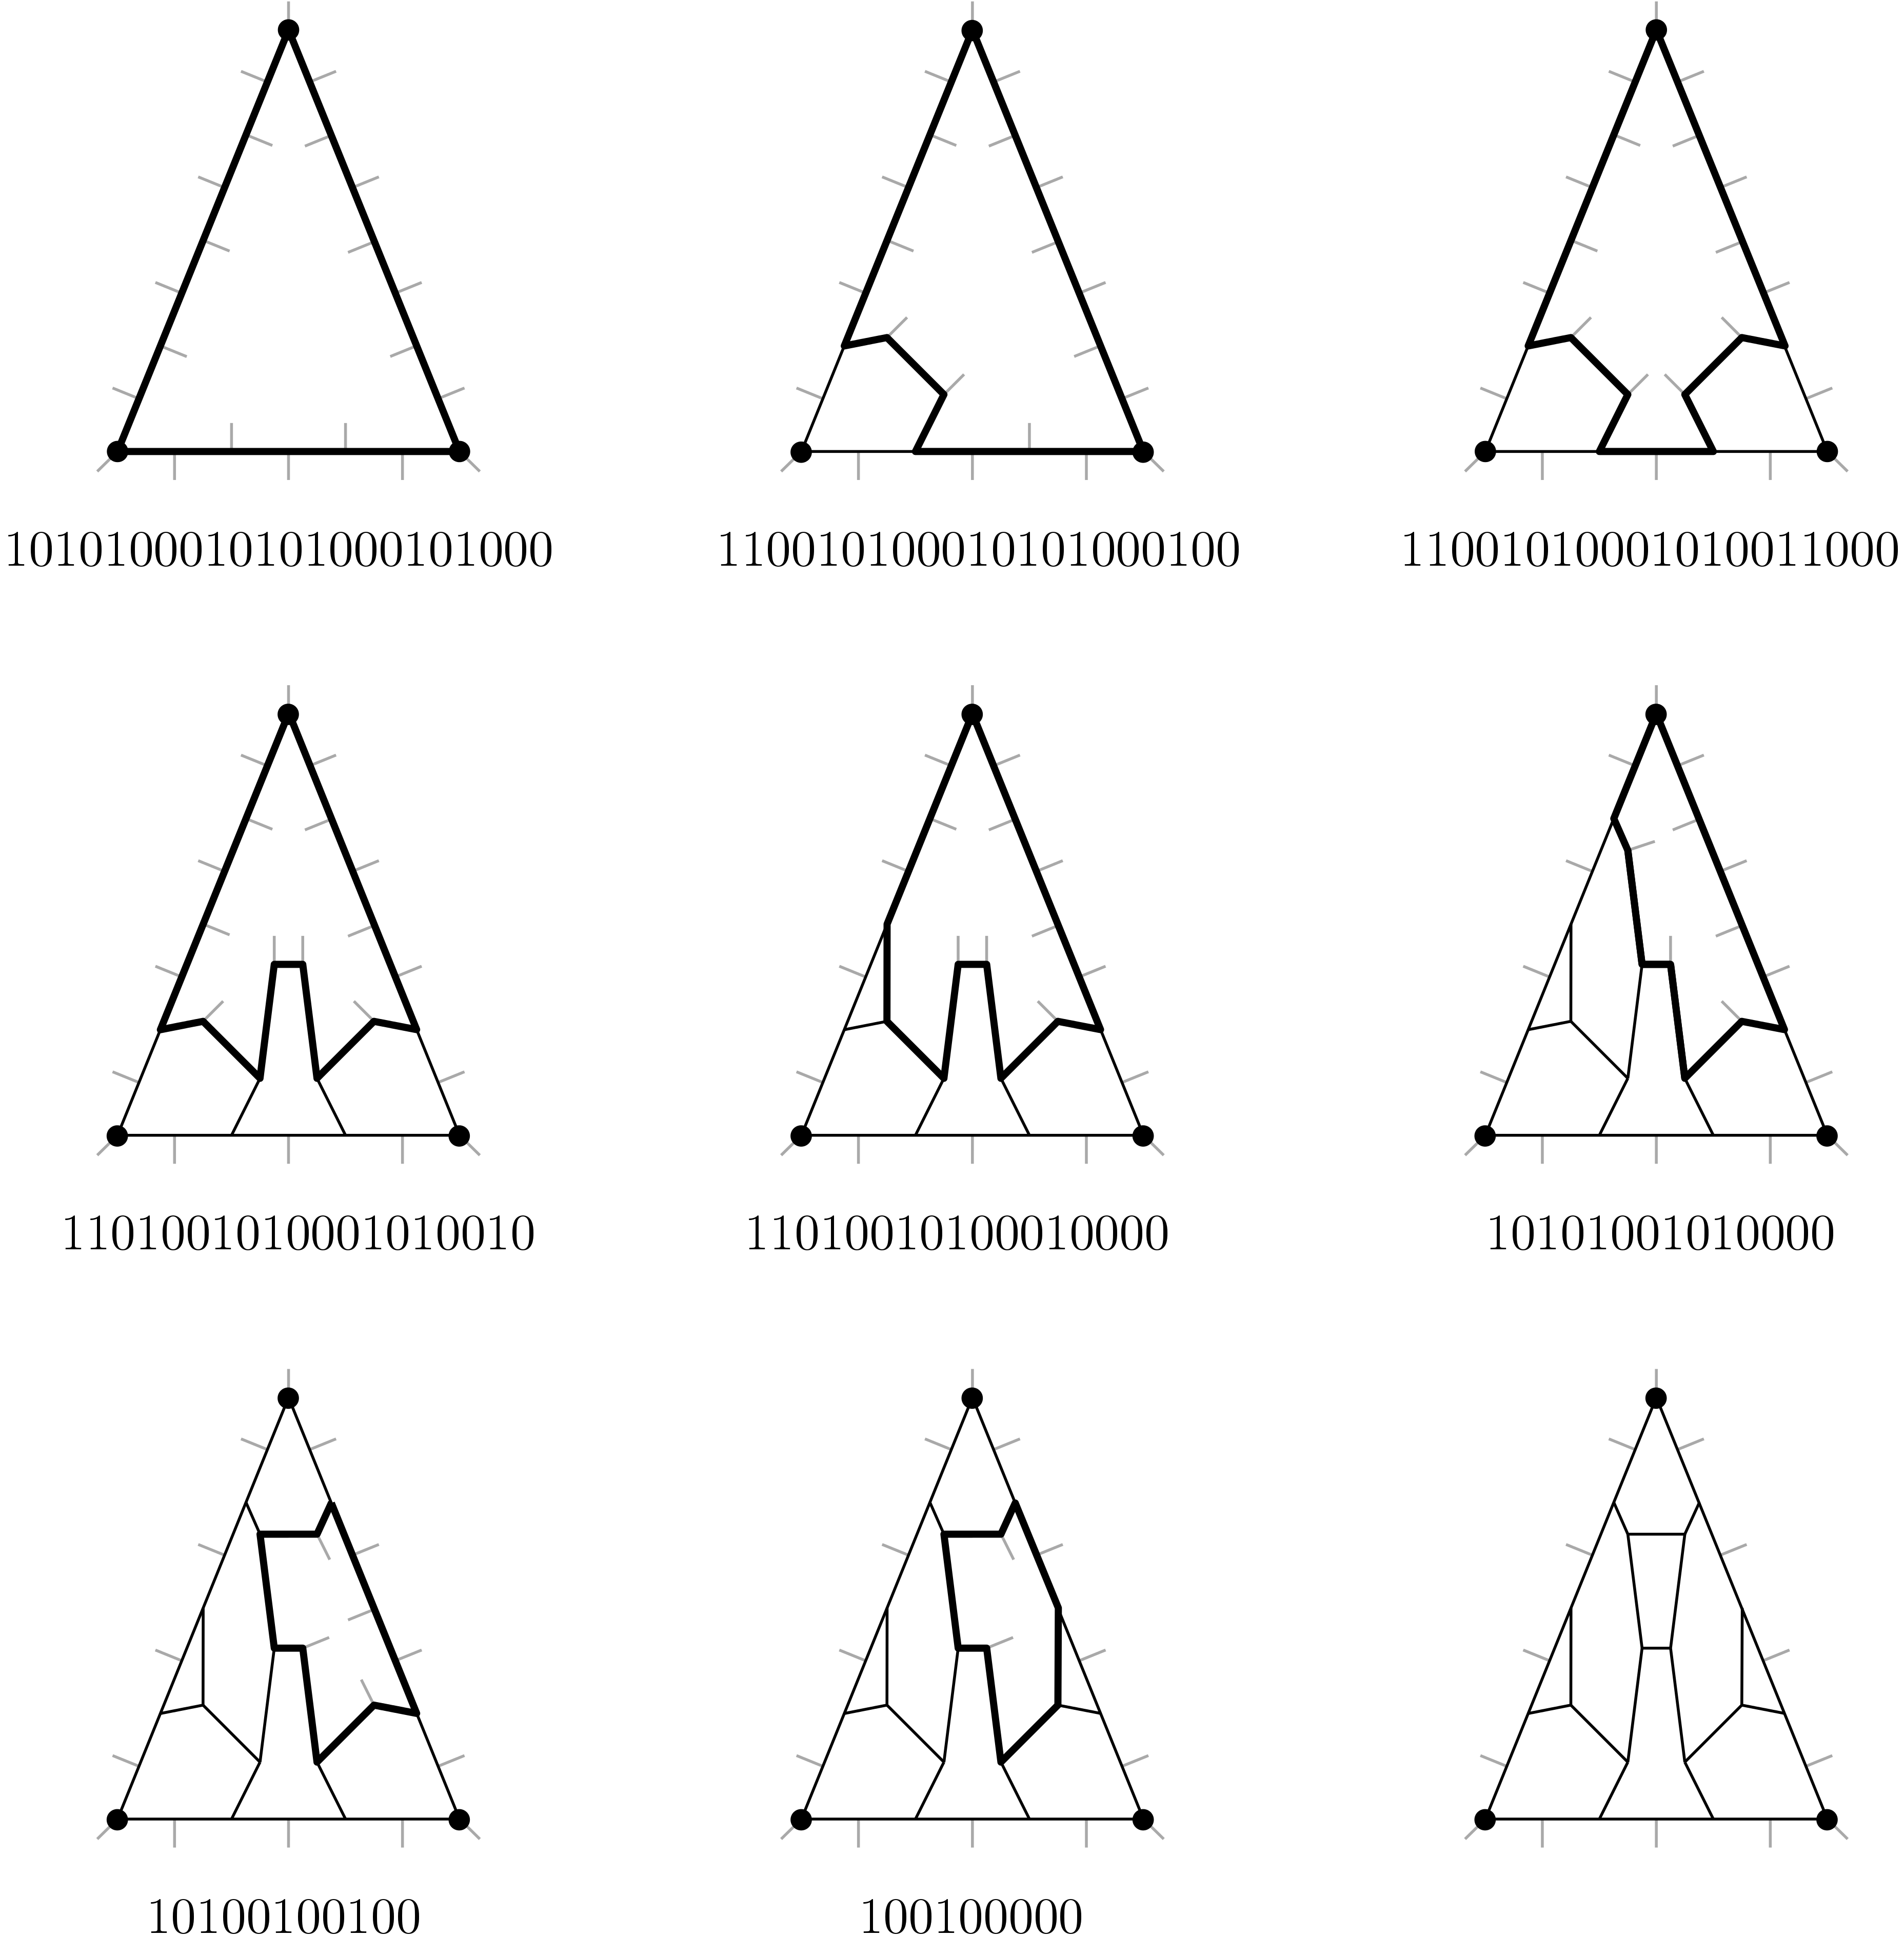
\includegraphics[width=\textwidth]{../img/reseni}
\caption{Možný postup vyplnění (4,4,3)$\lbrace$4,7$\rbrace$-triarku. Hodnota pod grafem vždy odpovídá reprezentaci aktuální, tučně zvýrazněné, hranice.}
\label{obr03:reseni}
\end{figure}

Pro jistotu poznamenejme, že pokud program hledaný graf nenašel, může, ale nemusí to znamenat, že neexistuje.

Podle předchozí kapitoly pro dokončení důkazu pro konkrétní dvojici $p$ a $q$ a nějaké přirozené $k$ potřebujeme tyto čtyři typy grafů:
\begin{description}
\item[(i)] ($k$, $k$, $k$),$Q$-triark;
\item[(ii)] ($k$, $k$, $k-1$),$Q$-triark;
\item[(iii)] ($mk$,$mk$,$x$),$Q\cup \lbrace 1\rbrace$-triark, kde je právě jedna stěna velikosti $l$;
\item[(iv)] prstenec, který dokáže spojit dva stejně velké, rovnostranné triarky.
\end{description}

Pro dané $k$ získáme grafy (i) a (ii) z řešítka hned. Pro zbylé je nutné pomoci si konstrukcí, která se ukázala jako úspěšná pro některé neutrální sekvence. O výsledcích získaných z programu píšeme v další kapitole. TODO odkaz?

Na graf (iii) se neumíme zeptat přímo, protože potřebujeme v grafu mít právě jednu stěnu délky $p_l$. Spojme proto stěnu s vnější stěnou triarku ručně a ptejme se na výplň vzniklých oblastí $A$ a $B$. Ke spojení použijeme $l$ kopií řetízku $R$, každý napojíme na jeden z vrcholů jádra a druhé konce spojíme s \uv{in} vrcholy základny triarku. V řetízku navíc fixujeme, ve které straně od něj budou mít které jeho vrcholy třetího souseda (znázorněno šedě v obrázku TODO odkaz). Konstrukce je obecná pro všechny přípustné hodnoty $l$, tedy není závislá na volbě $p$. Navíc není (při dobré volně R) vynucená ani příliš velká stěna, takže konstrukce může být obecná i pro všechny q (protože q je neutrální, tedy v ní musí být nenulová hodnota na pozici reprezentující stěnu velikosti alespoň 6, tvrzení \eqref{veta:posloupnosti}.



Podobnou konstrukci tvoříme i pro graf typu (iv). V tomto případě za pomoci řetízků spojujeme odpovídající vrcholy rovnostranných, stejně velkých triarků $T_1$ a $T_2$. Vzniknou dva typy oblastí - $C$ při rozích triarku a $D$ mezi odpovídajícími kusy stran triarků. Poznamenejme, že na obrázku je $T_2$ nakreslen "naruby" TODO lepší slovo?. 

Tyto konstrukce jsou v řešítku implementovány. Výsledný program tedy na vstupu očekává seznam velikostí stěn, které mohou tvořit neutrální posloupnost. Pokud pro daný seznam stěn existuje více neutrálních posloupností, využije program pro každý pomocný graf libovolnou z nich.

\begin{figure}[h!]\centering
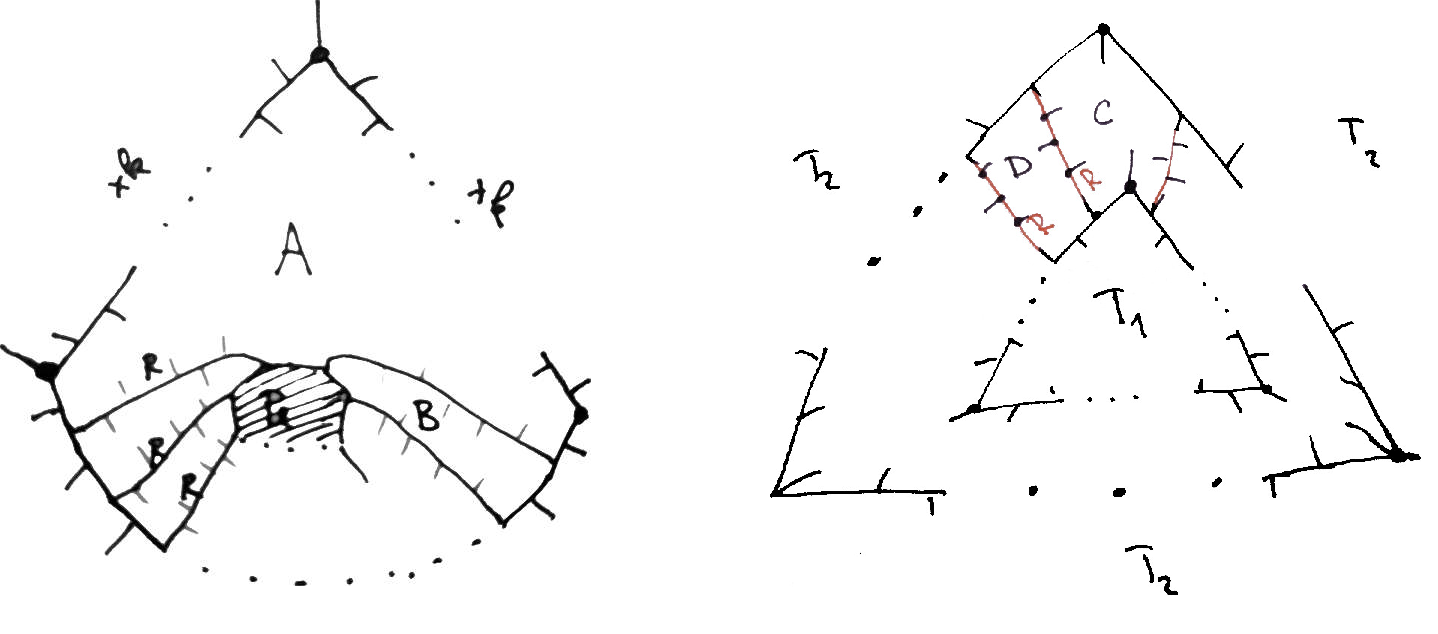
\includegraphics[width = \textwidth]{../img/iii+iv-construction}
\caption{Vlevo konstrukce grafu typu (iii), konkrétně ($xk$,$xk$,$l+1$)-triarku s jádrem velikosti $l$, vpravo konstrukce grafu typu (iv).}
\label{obr03:konstrukce}

\end{figure}

\section{Uživatelská dokumentace}


